\documentclass{standalone}
\usepackage{tikz}
\usepackage{verbatim}
\begin{document}
\pagestyle{empty}
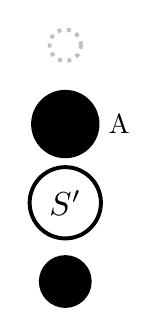
\begin{tikzpicture}

  % The graphic
  \node[draw,circle,scale=1.2, gray!50, dotted, fill=white, line width=0.5mm] (s_0) at (0,0) {};
  \node[draw,circle,scale=0.8, fill=black, line width=0.5mm, label=right:A] (a_0) at (0,-1) {$S,A$};
  \node[draw,circle,scale=1.2, fill=white, line width=0.5mm] (s_1) at (0,-2) {$S'$};
  \node[draw,circle,scale=0.8, fill=black, line width=0.5mm] (a_1) at (0,-3) {$A'$};
       
\end{tikzpicture}
\end{document}